\documentclass[sigconf]{acmart}

\usepackage{booktabs} % For formal tables
\usepackage{listings}
\usepackage{color}
\usepackage{courier}
% \usepackage[hyphenbreaks]{breakurl}

% Copyright
%\setcopyright{none}
%\setcopyright{acmcopyright}
%\setcopyright{acmlicensed}
\setcopyright{rightsretained}
%\setcopyright{usgov}
%\setcopyright{usgovmixed}
%\setcopyright{cagov}
%\setcopyright{cagovmixed}
\lstset{basicstyle=\ttfamily\footnotesize,breaklines=true}
\lstdefinelanguage{miniKanren}{
  language     = Lisp,
  morekeywords = {conde,fresh,run,run*,lambda,define,==,=/=,symbolo,numbero},
}

%Conference
\acmConference[CPS 452]{CPS 452: Emerging Programming Languages}{Fall 2019}{University of Dayton, Dayton, Ohio\ \ 45469---2160}
\acmYear{2019}
\copyrightyear{2019}

%\ I assume you are okay with being labled the editor since you are reviewing the draft.
\editor{Saverio Perugini}

\begin{document}
\title{Concurrent Implementation of the \\ Fast Fourier Transform in Kotlin}

\author{Benjamin W. Amato}
\affiliation{%
  \institution{Department of Computer Science}
  \institution{University of Dayton}
  \city{Dayton}
  \state{Ohio}
  \country{USA}
  \postcode{45469–0232}
}
\email{amatob1@udayon.edu}

\begin{abstract}
We present an implementation of the \textit{Cooley-Tukey Fast Fourier Transform} (\textit{FFT}) algorithm in the Kotlin programming language. The Cooley-Tukey algorithm structure, which partitions the input into two parts and recursively solves each partition, lends itself to parallelism. Kotlin's coroutines allow for the introduction of concurrency with minimal additional code through it's async and await operators. The utility of the FFT is shown by comparing the Discrete Fourier Transform, Fast Fourier Transform, and Concurrent Fast Fourier Transform when finding the power spectra of an audio file.
\end{abstract}
\keywords{FFT, Fast Fourier Transform, Koltin, coroutine, async, concurrent.}
\maketitle
\section{Introdution}
The Fourier Transform is function which converts a signal represent expressed as function of time into one expressed as a function of frequency. Since any periodic signal can be represented as a sum of sine waves, the frequency content of signal can be extracted using the Fourier Transform. The Fourier Transform is used in a number of signal processing applications including finding the power spectra of a signal, which will be demonstrated in this paper~\cite{PowerSpecta}.  The Discrete version of the Fourier Transform can be represented by the equation:
\[X_k = \sum_{n=0}^{N-1} x_n\cdot e^{-i2\pi k n/N}  \]
Each element of the \textit{Discrete Fourier transform} (\textit{DFT}) is the summation of each element in the input multiplied by a complex exponential number. This results in a computational complexity when solving the Discrete Fourier Transform of $\mathcal{O}(N^2)$. Cooley and Tukey demonstrated that this equation can be simplified by performing the Discrete Fourier Transform separately on portions of the input. The reduction of the DFT into the Cooley-Tukey Fast Fourier Transform (FFT) is shown below.
\[X_k = \sum_{n=0}^{N-1} x_n\cdot e^{-i2\pi k n/N}  \]
\[X_k = \sum_{m=0}^{N/2-1} x_{2m}\cdot e^{-i2\pi k 2m/N} + \sum_{m=0}^{N/2-1} x_{2m+1}\cdot e^{-i2\pi k (2m+1)/N}   \]
\[X_k = \sum_{m=0}^{N/2-1} x_{2m}\cdot e^{-i2\pi k 2m/N} + e^{-i2\pi k /N}\sum_{m=0}^{N/2-1} x_{2m+1}\cdot e^{-i2\pi k (2m)/N}   \]
Each summation is itself a Discrete Fourier Transform, allowing the DFT to be run on two smaller problems, making the resulting complexity be $2mathcal{O}(M^2)$ where $M = N/2$. This simplification can be applied to each smaller problem, halving the computation time each time and resulting in a total computational complexity of $\mathcal{O}(N\log{N})$.
\begin{figure}
    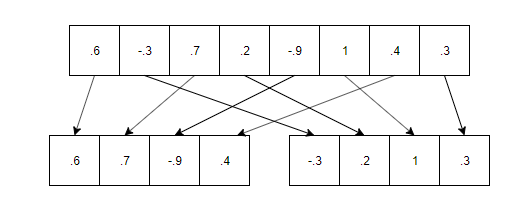
\includegraphics[scale=.6]{DiagramSeperate.PNG}
    \caption{FFT seperates every other element and applies again to each half.}
    \label{fig:my_label}
\end{figure}

\section{Implementation of the Discrete Fourier Transform in Koltin}
To implement the DFT in Koltin, first a representation of complex numbers is needed. Koltin does not have native support for complex numbers, so a \texttt{Complex} data object is needed.
\begin{lstlisting}[language=kotlin]
data class Complex(var real: Double, var imag: Double){}
\end{lstlisting}
By declaring the class as a data class, the Koltin compiler automatically creates some common methods, including the \texttt{equals()} and \texttt{toString()} methods. Utilizing Kotlin's operator overloading, common mathematical operators on Complex numbers were introduced. This allows users to use standard infix operators, such as \texttt{*}, \texttt{+}, and \texttt{/}, when dealing with complex numbers.
\begin{lstlisting}[language=kotlin]
operator fun plus(c: Complex): Complex {
        return Complex(real + c.real, imag + c.imag)
    }
    operator fun minus(c: Complex): Complex {
        return Complex(real - c.real, imag - c.imag)
    }
    operator fun times(c: Complex): Complex {
        return Complex(real * c.real - imag * c.imag, real * c.imag + imag * c.real)
    }

    operator fun times(d: Double): Complex {
        return Complex(real * d,imag * d)
    }

    operator fun div(c: Complex): Complex {
        val conj = Complex(c.real, - c.imag)
        val num = Complex(real, imag) * conj
        val denom = c * conj
        return Complex(num.real / denom.real, num.imag / denom.real)
    }
\end{lstlisting}
The DFT is used inside the FFT so it is placed inside a companion object for the \texttt{FFT} class. Companion objects allows the methods to be called directly form the class name, similarly to static methods in Java. The direct transcription of the DFT is shown below.
\begin{lstlisting}[language=kotlin]
fun dftComplex(values: List<Complex>): List<Complex>{
    var result :MutableList<Complex> = MutableList(values.size){Complex(0.0,0.0)}
    for((i, value) in result.withIndex()){
        for(j in values.indices){
            result[i] += eToNeg2PiITimes(i*j/result.size.toDouble()) * values[j]
        }
    }
    return result
}
\end{lstlisting}
The DFT loops through all elements in the input for evety output, adding that input times a complex exponential. The exponential is obtained from the \texttt{eToNeg2PiITimes()} helper function shown below. 
\begin{lstlisting}[language=kotlin]
private fun eToNeg2PiITimes(num: Double): Complex{
    val pi = 3.141593654
    // From Euler's Formula
    return Complex(Math.cos(2*pi*num), - Math.sin(2*pi*num))
}
\end{lstlisting}
This function calculates the value of the exponential using Euler's Formula, which states that $e^{-i\theta}$ can be found by taking $cos(\theta) - i\cdot sin(\theta)$. With this the Discrete Fourier Transform is complete.
\section{Implementing the Cooley-Tukey Fast Fourier Transform}
Using the structure of the DFT as a base, the Cooley-Tukey Fast Fourier Transform is implemented. The code for the FFT is shown below.
\begin{lstlisting}[language=kotlin]
private fun fftComplex(values: List<Complex>):List<Complex>{
    var result: MutableList<Complex> = MutableList(values.size){Complex(0.0,0.0)}
    //At 32 values, DFT is faster
    if(values.size <= 32){
        return dftComplex(values)
    }
    if(values.size % 2 != 0){
        return dftComplex(values)
    }
  
    val even = fftComplex(values.filterIndexed { index, _ -> index % 2 == 0 }, false)
    val odd = fftComplex(values.filterIndexed { index, _ -> index % 2 == 1 }, false)
    for (i in odd.indices) {
        var secondHalf = i + odd.size
        result[i] = even[i] + odd[i] * eToNeg2PiITimes(i.toDouble() / values.size)
        result[secondHalf] = even[i] + odd[i] * eToNeg2PiITimes(secondHalf.toDouble() / values.size)
    }
    return result
}
\end{lstlisting}
The Cooley-Tukey FFT relies on there being an even number of elements in the input so that the FFT can be divided evenly into equal halves. When there are not an even number of elements, the much slower DFT algorithm is used since it has no restrictions on input size. Similarly, there is some overhead in creating and running two sub-problems, so for very small inputs the DFT is faster and is relied upon. The core of this Koltin implementation relies on using Kotlin's \texttt{List} filters to separate every other element in the input. These separated elements are then processed using the the FFT and combined to form the output. The output can be thought of as two pieces of the FFT concatenated to each other, the first being the even FFT plus the odd FFT times a complex exponential, and the second being the even FFT plus the odd FFT times a different complex exponential. 
\section{Introducing Concurrency}
Using Kotlinx's recently introduced coroutine library, concurrency can be added to the FFT. Coroutines act as lightweight threads, allowing many to be spawned without causing major performance problems. Since the computation of the even and odd FFT terms is independent of each other, Kotlin's async operation can be used to spawn a coroutine for the even turn, while the current co-routine calculates the odd terms.
\begin{lstlisting}
if(spawn && values.size > 10000){
    val even = GlobalScope.async { fftComplex(values.filterIndexed{ index, _ -> index%2 == 0}, true)}
    runBlocking {
        val odd =  fftComplex(values.filterIndexed{index, _ -> index%2 == 1}, true)
        for(i in odd.indices) {
            var secondHalf = i + odd.size
            result[i] = even.await()[i] + odd[i] * eToNeg2PiITimes(i.toDouble()/values.size)
            result[secondHalf] = even.await()[i] + odd[i] * eToNeg2PiITimes(secondHalf.toDouble()/values.size)
        }
    }
    return result
}
\end{lstlisting}
A new parameter, spawn, is introduced to determine if additional co-routines should be created. Additionally, since co-routines have some overhead in their creation, even though it is less than full threads, there is a lower limit on the size of the input where adding concurrency help. Though testing, a input size of less than 10,000 generally causes the concurrent process to be slower than the non concurrent. When spawn if false or the size of the input list is less than 10,000 the non-concurrent code presented in the last section is utilized instead.
To obtain the result from the \texttt{async} function, \texttt{await} can be called. \texttt{Await} blocks the current coroutine until the \texttt{async} code returns and must be placed inside a \texttt{runBlocking} code block. \texttt{RunBlocking} ensures that the current coroutine can be suspended to wait for \texttt{async} function to complete. Since generally the even and odd FFTs take a similar time to execute, there should be little time wasted waiting on the asynchronous even FFT to complete.
\begin{table}
  \caption{Time to run DFT and FFT.}
  \label{tab:dtf}
  \begin{tabular}{rrr}
    \toprule
    Number & DFT(ms) & FFT(ms)\\
    \midrule
    64 &  0 & 1\\
    128 &  2 & 1\\
    256 &  6 & 3\\
    512 &  24 & 4\\
    1024 &  114 & 8\\
    2048 &  397 & 17\\
    4096 &  1664 & 36\\
    8192 &  6798 & 72\\
    16384 &  27354 & 145\\
    32768 &  113108 & 295\\
  \bottomrule
\end{tabular}
\end{table}
\section{Analysis of the FFT}
The utility of utilizing the FFT can be seen by examining the time differential between the FFT and the DFT. The time values for different size inputs are shown above in Table 1. At very small sizes, less than 128 values, the difference is minimal, but as the size of the input increases the time difference increases. When the size of the input is 32768 value, the max size tested, the DFT takes over 700 times as long as the FFT, with a time of almost two minuets compared to the 160 milliseconds of the FFT.
\begin{table}
  \caption{Time to run FFT with and without Concurrency.}
  \label{tab:dtf}
  \begin{tabular}{rrr}
    \toprule
    Number & Non-Concurrent(ms) & Concurrent(ms)\\
    \midrule
    1024 &  9 & 9\\
    2048 &  17 & 29\\
    4096 &  36 & 37\\
    8192 &  75 & 76\\
    16384 &  154 & 90\\
    32768 &  299 & 152\\
    65536 &  626 & 180\\
    131072 &  1326 & 311\\
    262144 &  2688 & 805\\
  \bottomrule
\end{tabular}
\end{table}
\subsection{Analysis of Concurrency}
When concurrency is introduced there is again a speedup in the FFT. Since concurrency is ignored at lower input sizes, the times are near identical. At larger input sizes, the use of concurrency allows for speedup to 2 to 4 times on the 4 core, 8 thread machine the code was tested on. Better familiarity with the Koltin concurrency operations could allow for additional improvements.

\subsection{Shortcomings of the Cooley-Tukey Algorithm}
All the comparisons in Table 1 and Table 2 were done on power of two sized inputs. Since the Cooley-Tukey algorithm must divide each stage into equal sized portions, non-power of two inputs are much slower. At some point, a odd number input will be reached if the starting size is not a power of two, causing the the standard DTF to be run. While there are some mitigation methods for this, including dividing the input into more than 2 sub-problems or using zero-padding to increase the input to a power of two, these methods are not part of the standard Cooley-Tukey algorithm and were not implemented here~\cite{SplitRadix}\cite{zero-padding}.
\begin{figure}
    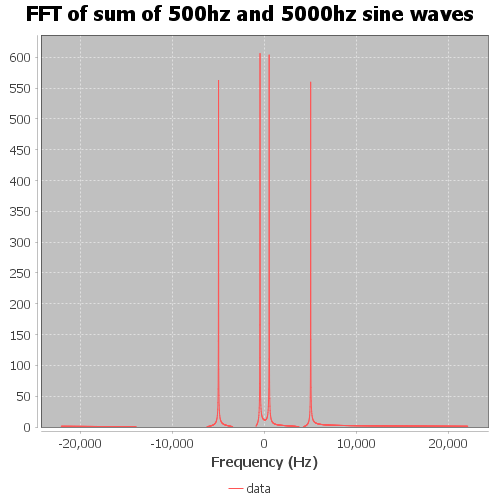
\includegraphics[scale=.5]{5500hz.png}
    \caption{Fourier Transform of 500hz and 5500hz sine wave.}
    \label{fig:my_label}
\end{figure}
\section{Use in Power Spectra}
The utility of the FFT can be seen when finding the power spectra of a signal. The power spectra of signal is the amount of power in a signal at different frequencies. It has a number of use cases, including visualizing what frequencies signals are at when receiving a broadband signal. To simulate this, two sine waves, one at 500hz and one at 5000hz, were added together to represent data being send at two separate frequencies over a broadband signal. The receiving device would not know where the data is located on the spectrum. By taking the FFT of the signal, two spikes, as seen in Figure 2, appear. These spikes are at 500hz and 5000hz. Using this, the receiving device can tune itself the the correct frequencies and receive the data.


\bibliographystyle{ACM-Reference-Format}
\bibliography{FFT.bib}

\end{document}